\documentclass[10pt]{article}
\usepackage[polish]{babel}
\usepackage[utf8]{inputenc}
\usepackage[T1]{fontenc}
\usepackage{graphicx}
\usepackage[export]{adjustbox}
\graphicspath{ {./images/} }
\usepackage{amsmath}
\usepackage{amsfonts}
\usepackage{amssymb}
\usepackage[version=4]{mhchem}
\usepackage{stmaryrd}

\title{Akademia \\
 Pomorska \\
 w Stupsku }

\author{}
\date{}


\begin{document}
\maketitle
\begin{center}

\includegraphics[max width=\textwidth]{2024_11_21_823cc8b405444b8ad8bfg-1}
\end{center}

\begin{center}

\includegraphics[max width=\textwidth]{2024_11_21_823cc8b405444b8ad8bfg-1(2)}
\end{center}

\section*{LIGA MATEMATYCZNA \\
 im. Zdzisława Matuskiego \\
 FINAŁ 21 kwietnia 2022 \\
 SZKOŁA PODSTAWOWA \\
 klasy VII - VIII}
\section*{ZADANIE 1.}
Cyfrą dziesiątek liczby trzycyfrowej \(A\) jest 8 . Jeżeli tę cyfrę przestawimy na miejsce cyfry jedności, to otrzymamy liczbę o 9 mniejszą od liczby \(A\). Jeżeli przestawimy 8 na miejsce cyfry setek, to otrzymamy liczbę o 630 większą od liczby \(A\). Wyznacz liczbę \(A\).

\section*{ZADANIE 2.}
Znajdź najmniejszą liczbę naturalną zapisaną tylko za pomocą zer i jedynek, podzielną przez 45.

\section*{ZADANIE 3.}
Wokół okrągłego stołu siedzi 13 osób. Każda z nich ma na talerzu inną liczbę pierogów. Czy można znaleźć dwie sąsiednie osoby, które w sumie mają parzystą liczbę pierogów? Odpowiedź uzasadnij.

\section*{ZADANIE 4.}
Adam pomnożył sześć kolejnych liczb całkowitych dodatnich i uzyskał iloczyn \(A\). Bartek też pomnożył sześć kolejnych liczb całkowitych dodatnich, ale zaczął od liczby o 1 większej niż Adam. Otrzymał liczbę \(B\). Wyznacz najmniejszy czynnik iloczynu Bartka, jeżeli \(\frac{A}{B}=\frac{5}{6}\).

\section*{ZADANIE 5.}
W kwadracie o boku o długości 4 cm umieszczono prostokąt tak, jak na rysunku. Oblicz obwód tego prostokąta.\\
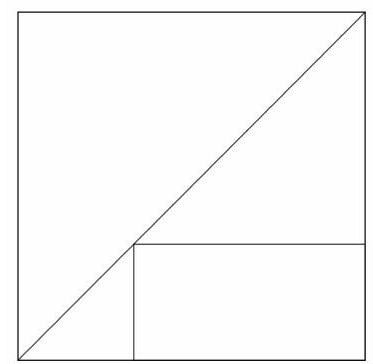
\includegraphics[max width=\textwidth, center]{2024_11_21_823cc8b405444b8ad8bfg-1(1)}


\end{document}